\section{Introduction}
Collective dynamics is an interesting research area in many fields of study ranging from natural science, mathematics, to social science. The reasons for which are also far and wide, ranging from relevant practical applications to plain curiosity. Collective dynamics, as the name suggests, involve interactivity of a collection of objects \cite{schweitzer1997self} (e.g. crowds of pedestrians, flocks of birds, social systems etc.). These moving parts -- under the right conditions -- may exhibit a self-organizing characteristic that emerge out of the local interaction of the moving parts \cite{yates2012self}. Examples of such collective behavior include oscillatory behavior of dense crowds \cite{gu2025emergence}, stop-and-go waves from traffic flows and crowd dynamics \cite{yeo2009understanding,chraibi2016force}, formation of opinions in a society \cite{moussaid2013opinion} to name a few.
\begin{figure}[H]
    \centering
    \begin{subfigure}{.49\textwidth}
        \centering
        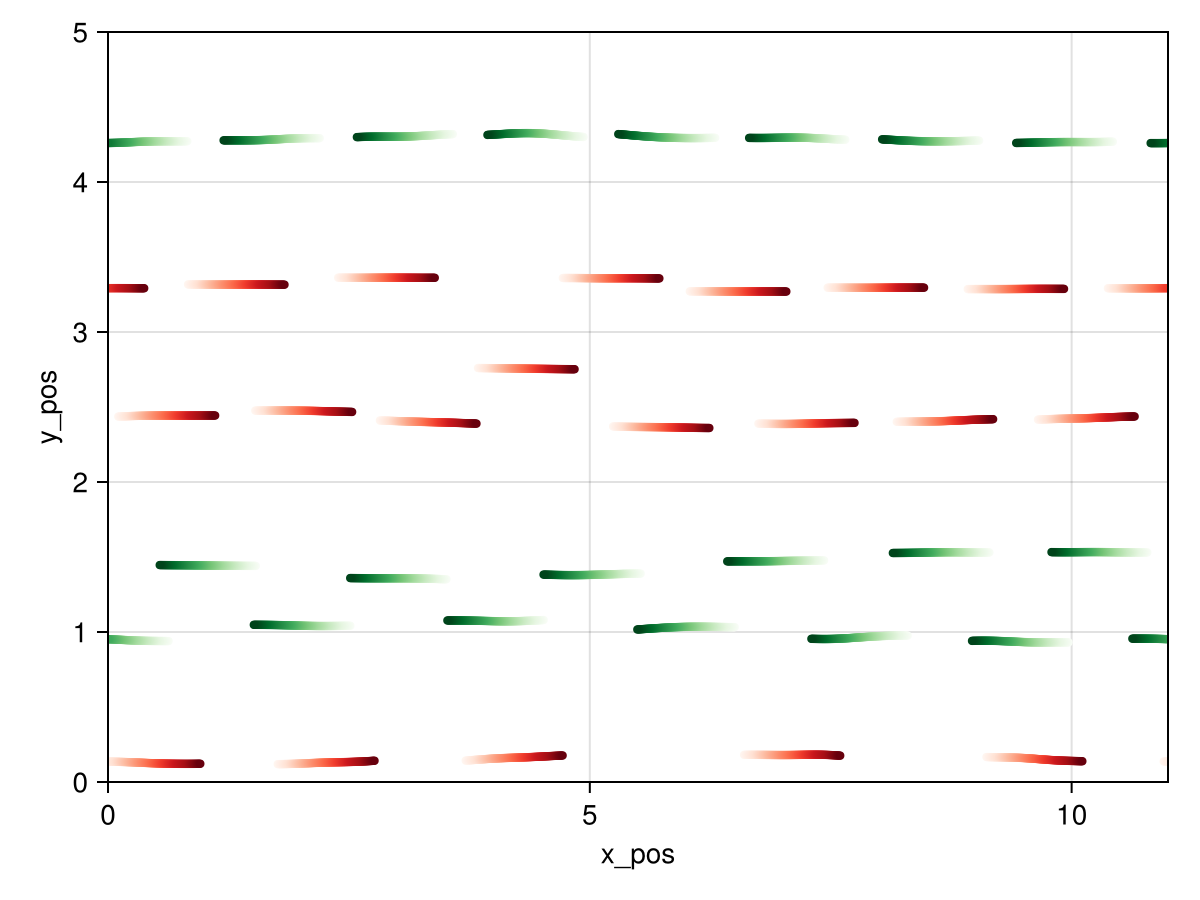
\includegraphics[width=\linewidth]{figures/counter_40_2flow_10000.png}
        \caption{Lane formation for counter flows}
        \label{plot:example_cross}
    \end{subfigure}
    \begin{subfigure}{.49\textwidth}
        \centering
        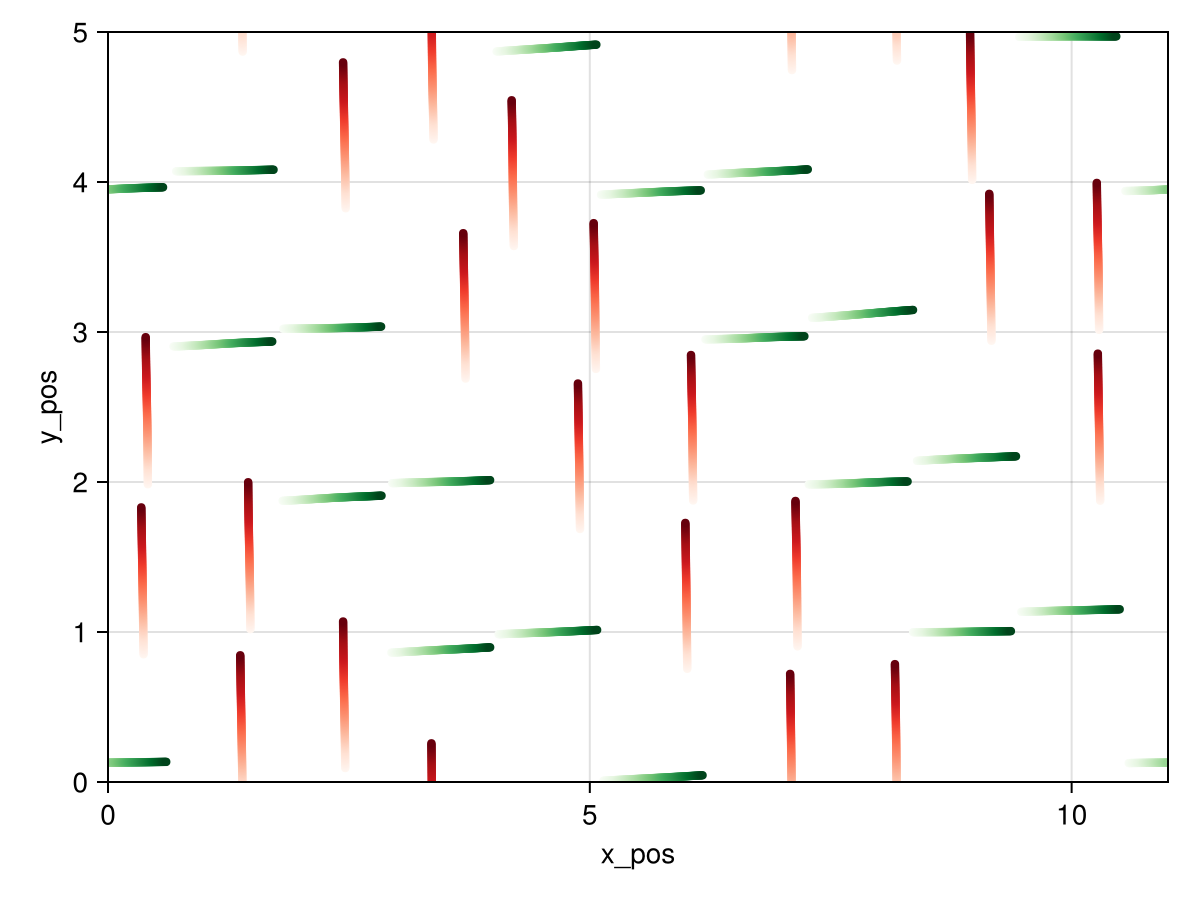
\includegraphics[width=\linewidth]{figures/cross_40_2flow_10000.png}
        \caption{Stripe formation for cross flows}
        \label{plot:example_counter}
    \end{subfigure}
    \caption{Examples of collective phenomenon in pedestrian dynamics. The colors differentiate the pedestrians based on their desired directions.}
    \label{plot:examples}
\end{figure}
\textbf{Microscopic Model for Pedestrian Dynamics}

In this study, we pay our attention to the collective behavior observed in pedestrian models using the idea from Helbing's social force model (SFM) \cite{helbing1995social}. The movement of pedestrians arises from a combination of \textit{social forces} that affect them individually into taking certain directions as a result. Depending on the spacial boundaries, pedestrian interactivity, and their direction of movement, one can observe self-organizing patterns (see \autoref{plot:examples}) such as lane formation for counter-flows i.e. when two groups of pedestrians move in opposite directions (e.g. left-to-right and right-to-left), and stripe/band formation for cross-flows i.e. when two groups of pedestrians move in perpendicular directions (e.g. left-to-right and up-to-down) \cite{Mullick_2022,sieben2017collective,khelfa2021initiating,tordeux2022multi}. These macroscopic patterns emerge out of the microscopic interaction between individual pedestrians, serving as one of the examples of emergent phenomenon within complex systems \cite{fromm2004emergence}.

\textbf{Port-Hamiltonian Systems Approach}

It is understandable that due to the involved interactivity and self-propelled behavior, the resulting nonlinear dynamics poses quite a challenge in modeling and controlling pedestrian systems \cite{appertrolland2024modellingvehiclepedestriancollective}. In this thesis, we will attempt to describe the  dynamics through a modeling approach known as port-Hamiltonian systems (PHS), giving an energy-based perspective to describe the overall behavior of the model. 

Port-Hamiltonian systems theory is a relatively new, yet promising, paradigm to model nonlinear physical systems \cite{van2014port,duindam2009modeling}. Extending the classical Hamiltonian mechanics to allow modeling of open systems, as it allows systems to interact with other systems through ports that serve as inputs and outputs for the flow of energy between them. The framework is used for control for nonlinear multiphysics systems as well \cite{van2024port,van2004port}. Microscopic models are described by finite-dimensional PHS, which has been used to model various multi-agent systems including consensus and opinion formation \cite{van2013port,xue2019opinion}, swarm behavior \cite{matei2019inferring}, multi-input multi-output agent systems \cite{sharf2019analysis}. Whereas macroscopic systems are modelled using infinite-dimensional PHS, these include fluid dynamic models \cite{rashad2021port}, and macroscopic traffic flow models \cite{bansal2021port}. To account for uncertainties in the system, the theory of port-Hamiltonian systems also extends to stochastic cases \cite{cordoni2022stochastic}, involving stochastic car-following models \cite{rudiger2024stability}, and more generally self-driven agent models \cite{ehrhardt2024collective}.



\textbf{Overview and Objectives}

The objective of this thesis is to represent the dynamics of the microscopic force-based pedestrian model through the port-Hamiltonian formulation. We establish that the port-Hamiltonian formulation is interchangeable with the agent-based formulation, signifying that the model possesses Hamiltonian structure. Once this is established, we devise that the Hamiltonian can be used as a measure to quantify macroscopic behavior of the overall model; and observe the relationship between the self-organized collective behavior and the overall system energy, i.e. the Hamiltonian. Next, we move on to the stochastic case, and subject the dynamics to additive noise. We investigate the dynamics of the stochastic port-Hamiltonian formulation of the model and observe its impact on the Hamiltonian measure as well as on the macroscopic collective behavior.

To simulate the models, we keep in mind that the numerical method should be considerate of the energy of the system, and thus we compare different solvers and establish that symplectic methods are best suited for our port-Hamiltonian model. The agent-based models are made using the Julia programming language with \texttt{Agents.jl} \cite{Agents.jl} package. To add more flexibility and to easily compare a variety of different numerical solvers, we also make use of the \texttt{DifferentialEquations.jl} \cite{rackauckas2017differentialequations} package to construct our solvers, this proved useful paricularly for the stochastic port-Hamiltonian case.




% \begin{lstlisting}[language=Julia]
%     print(hello)
% \end{lstlisting}<